\documentclass{acmsiggraph}
\usepackage[english,french]{babel}
\usepackage[T1]{fontenc}
\usepackage[latin1]{inputenc}
\usepackage{float, enumitem, footnote, multirow,subfig}
\usepackage{amsmath, amsthm, amssymb}
\usepackage[linesnumbered,ruled,vlined]{algorithm2e}
\usepackage{microtype}
\usepackage{lmodern}
\graphicspath{{../figures/}}

\newcommand\mycommfont[1]{\footnotesize\ttfamily{#1}}
\SetCommentSty{mycommfont}

\title{Project report \\
Machine Learning with Kernel Methods}

\author{Maha ELBAYAD \\
\large{Ecole Normale Superieure de Cachan - Master MVA}\\
\\\texttt{maha.elbayad@student.ecp.fr}}
\pdfauthor{Maha ELBAYAD}

\DeclareMathOperator\sign{sign}
\DeclareMathOperator\diag{diag}
\DeclareMathOperator\sigmoid{sigmoid}
\newcommand{\1}{\mathbf{1}}
\newcommand{\0}{\mathbf{0}}
\newcommand{\p}{\mathbb{P}}

\begin{document}
\maketitle

\section{Introduction}
This project aims at implementing a kernel based method from scratch to train a classifier on the MNIST dataset. We focused solely on variants of support vector machines.
\section{Outline}
We distinguish three different phases, first the pre-processing of the training samples (noise filtering, scaling, skew correction...) to enhance the quality of the images. The second main task is the features extraction where we design other features than the raw pixel intensities and choose appropriate kernels.Finally, the third phase tackles the optimization problem and prepare the classifier outputs for prediction.

\section{Pre-processing}
Our training set $\mathcal T=\{(x^{(i)},y^{(i)})\}_{1\leq i\leq m}$ consists of 5000 gray-scale $28\times28$ images distributed quite evenly among the 10 classes $\{0,1,...,9\}$. We experimented with skew correction via Hough transform so that we vertically align the dominant line.
\begin{figure}[H]
\centering
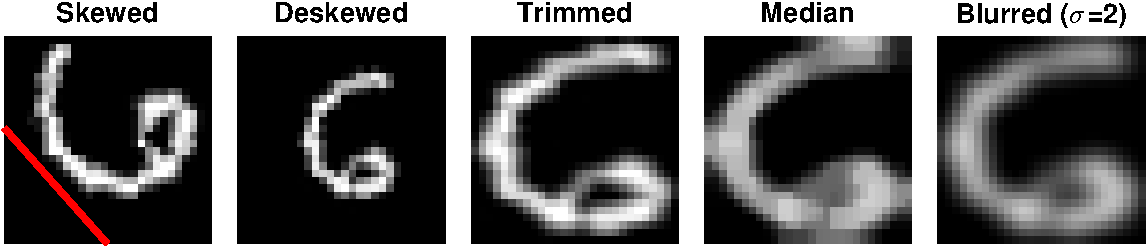
\includegraphics[width=8cm]{prep}
\end{figure}
Another pre-processing that improves the performance of our classifier is trimming the image black border as shown above. Afterwards, we either apply the median filter to denoise the image or the Gaussian blur to lessen the variance within each class. The final pixel intensities are adjusted in $[0,1]$ and with this pre-processing, normalizing the features globally doesn't improve the learning performance.  

\section{Features extraction}
\subsection{HOG features}
In order to include information about the image gradients, we append HOG features (histograms of oriented gradients) to the raw pixels . They can be seen as a nonlinear function of the edge orientations: we first evaluate the vertical and horizontal gradients of the image and pool them into local neighborhoods to remove sensitivity to exact localization of the edges. For each block of size $b\times b$ we compute an n-bins histogram of the gradient orientations and the final feature would be the concatenation of all histograms

\subsection{The kernels}
For the raw and HOG features we tested the following kernels:\\
\vspace{5pt}\\
\begin{tabular}{r|l ||c}
Linear & $K(x,y)=x^ty$ & Raw, HOG\\
RBF & $K_\sigma(x,y) = \exp(-x^ty/(2\sigma^2))$ & Raw, HOG\\
Poly & $K_d(x,y) = (1+x^ty)^d$ & Raw\\
$\chi_2$ & $K(x,y) = \sum_i(x_i-y_i)^2/(x_i+y_i)$ & HOG\\
Intersection & $K(x,y) = \sum_i\min(x_i,y_i)$ & HOG\\
\end{tabular}
\vspace{10pt}\\
Our implementation of those kernels is straightforward, thus the intersection and $\chi_2$ kernels are computationally expensive which hinder their efficiency although they're proven suitable for the HOG features.

\section{Support vector machines}
\subsection{Sequential Minimal Optimization (SMO)}
We wish to solve the QP dual problem of the regularized SVM:
\begin{equation}
\label{QP1}
\tag{QP1}
\begin{aligned}
%& \underset{\alpha}{\text{maximize}} & & W(\alpha) = \sum_{i=1}^m  \sum_{j=1}^m y^{(i)}y^{(j)}\alpha_i\alpha_jK(x^{(i)},x^{(j)}) \\
& \underset{\alpha}{\text{maximize}} & & W(\alpha) = \1^t\alpha - \frac{1}{2}\alpha^tH\alpha\\
& \text{subject to} & & \0\preceq \alpha \preceq C\1\\
& & & \alpha^tY = 0
\end{aligned}
\end{equation}
Where $Y = [y^{(1)},...,y^{(m)}]$ and $H = \diag(Y)K \diag(Y)$\\
For a vector $x$, we will predict:
\[\hat y(x) = \sign f(x) = \sum_{i=1}^m\alpha_iy^{(i)}K(x^{(i)},x)+b\]
A point is optimal if and only if the KKT conditions are fulfilled:
\begin{equation}
\begin{aligned}
\alpha_i=0&\Rightarrow &y^{(i)} f(x^{(i)}) \geq 1\\
\alpha_i\in (0,C)&\Rightarrow& y^{(i)} f(x^{(i)}) = 1\\
\alpha_i=C&\Rightarrow &y^{(i)} f(x^{(i)}) \leq 1\\
\end{aligned}
\tag{KKT}
\label{KKT}
\end{equation}
We implemented a simplified version of the SMO algorithm to solve (\ref{QP1}):\\

Repeat until convergence:
\begin{enumerate}
\item Select a violating term $\alpha_i$ i.e doesn't satisfy (\ref{KKT})
\item optimize $W(\alpha)$ with respect to $\alpha_i$ and a randomly selected term $\alpha_j$ while the other components are fixed.
\end{enumerate}

We consider that the algorithm has converged if $\alpha$ remains unchanged after a few iterations (cf. full algorithm in appendix).

Other intricate heuristics to select the most violating pair $(\alpha_i,\alpha_j)$ or a larger working selection were tested, but this version of SMO is sufficiently efficient.

\subsection{Multiple kernel learning (MKL)}
Given a set pf base kernels $\{K_k\}_{1\i\leq n}$, the objective of linear MKL is to jointly learn the SVM parameters and the linear combination of the base kernels:
\[K = \sum_{i=1}^nd_iK_i\]
The new $QP$ problem is:
\begin{equation}
\label{QP2}
\tag{QP2}
\begin{aligned}
& \underset{\alpha}{\text{maximize}} & & \1^t\alpha - \frac{1}{2}\sum_{i=1}^n
d_i\alpha^tH_i\alpha + \frac{\lambda}{2}\|d\|_2^2\\
& \text{subject to} & & \0\preceq \alpha \preceq C\1\\
& & & \alpha^tY = 0
\end{aligned}
\end{equation}
where for each kernel $H_i= \diag(Y)K_i\diag(Y)$. SMO is suitable to solve this new problem as well (cf. full algorithm in appendix)

\section{Experiments and results}
To compare our models we considered k-fold cross-validation $(k=5)$ so that all observations are used for both training and validation, in the following we report both the k-fold estimated accuracy and the Kaggle leader-board score.
\subsection{One vs One}
The default SVM algorithm solves for binary classifiers, and since our problem is a multi-class classification (10 classes) we consider all possible classifiers between two classes (a total of ${10 \choose 2}=45$)
\subsection{One vs Rest}
For each class we learn a classifier where all the remaining classes are considered as one class. In this setting the positive class is a minority; to weight out the imbalance effect we consider two different regularization parameters per class $(C_+ = \beta C_-,\:\beta>1)$
\subsection{Final prediction}
With either one vs. one or one vs. rest strategy we end up with multiple scores for each observation. To combine those scores and output a final prediction we use the following:
\begin{enumerate}[label=$\bullet$]
\item One vs. one: each classifier cast a vote in the predicted class and we outputs the class with the most votes.
\item One vs. rest: in order to compare the 10 scores we learn the posterior class probability for each class using Platt's scaling technique:
\[\p(y=1|x) \approx p_{a,b}(s) \equiv \sigmoid(-(as+b))\]
where s is the SVM score and $a,b$ are optimized via logistic regression.
\end{enumerate}
\subsection{Results}
\begin{table}[H]
\centering
\resizebox{.5\textwidth}{!}{%
\begin{tabular}{|l|l|l|l|}
\hline
Kernel & parameters & Acc(1) & Acc(2)\\
\hline
Raw(linear) & $C_-=10 , \beta =1$ & 87.30\% & \\
Raw(poly, $d=3$) & $C_-=10 , \beta =1$ & 95.80\% & \\
Raw(poly, $d=5$) & $C_-=10 , \beta =1$ & 95.10\% & \\
Raw(rbf, $\sigma=4$)   & $C_-=10, \beta =2$ & 95.70\% & \\
Raw(rbf, $\sigma=7$)   & $C_-=10, \beta =2$ & 96.10\% & 95.42\%\\
Raw(rbf, $\sigma=10$)   & $C_-=10, \beta =2$ & 95.90\% & \\
\hline
HOG(linear)   & $C_-=10, \beta =1$ & 92.30\% & \\
HOG(intersection)   & $C_-=10, \beta =1$ & 93.70\% & \\
HOG(rbf, $\sigma=2$)   & $C_-=10, \beta =1$ & 96.10\% & \\
HOG(rbf, $\sigma=4$)   & $C_-=10, \beta =1$ & 96.00\% & \\
\hline
$K_1$= Raw(rbf, $\sigma=7$)   & \multirow{3}{*}{$C_-=10, \beta =2$} & \multirow{3}{*}{96.90\%} & \\
$K_2$= HOG(rbf, $\sigma=4$)   &                                  &         & \\
K = $K_1\odot K_2$   &                                  &         & \\
\hline
$K_1$= Raw(rbf, $\sigma=7$)   & \multirow{8}{*}{$C_-=10, \beta =3$} &  & \\
$K_2$= HOG(rbf, $\sigma=4$)   &                                  &         & \\
$K_3$= HOG(linear)   &                                  &         & \\
$K=K_1\odot(K_2+K_3+K_2\odot K_3)$   &                                  &         & \\
with blurring and deskewing   &                                  &       97.10\%  &  97.26\% \\
without blurring nor deskewing   &                                  &       97.00\%  & 97,08\% \\
without trimming   &                                  &       94.90\% & \\
MKL $\{K_1,K_2,K_3\}$   &                             &       97.20\% & 96.90\% \\

\hline
\end{tabular}}
\caption{Acc(1): k-fold accuracy - Acc(2): Kaggle accuracy}
\end{table}
\subsubsection{Best performance statistics}
\begin{figure}[H]
\centering
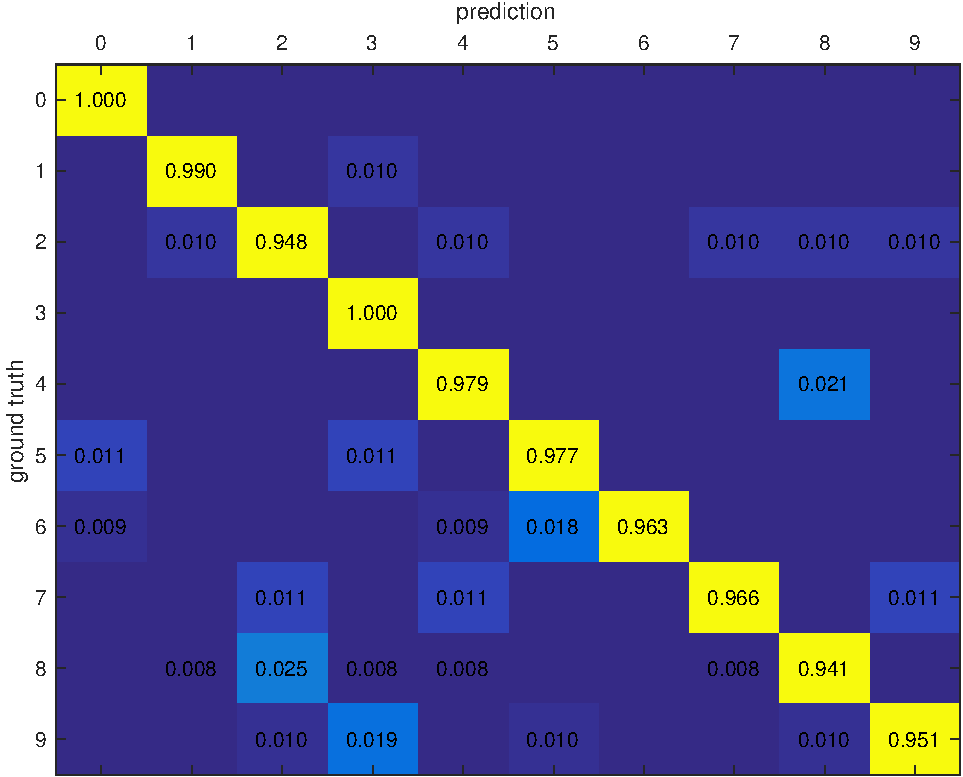
\includegraphics[width=7cm]{best_cf}
\end{figure}
\begin{figure}[H]
\centering
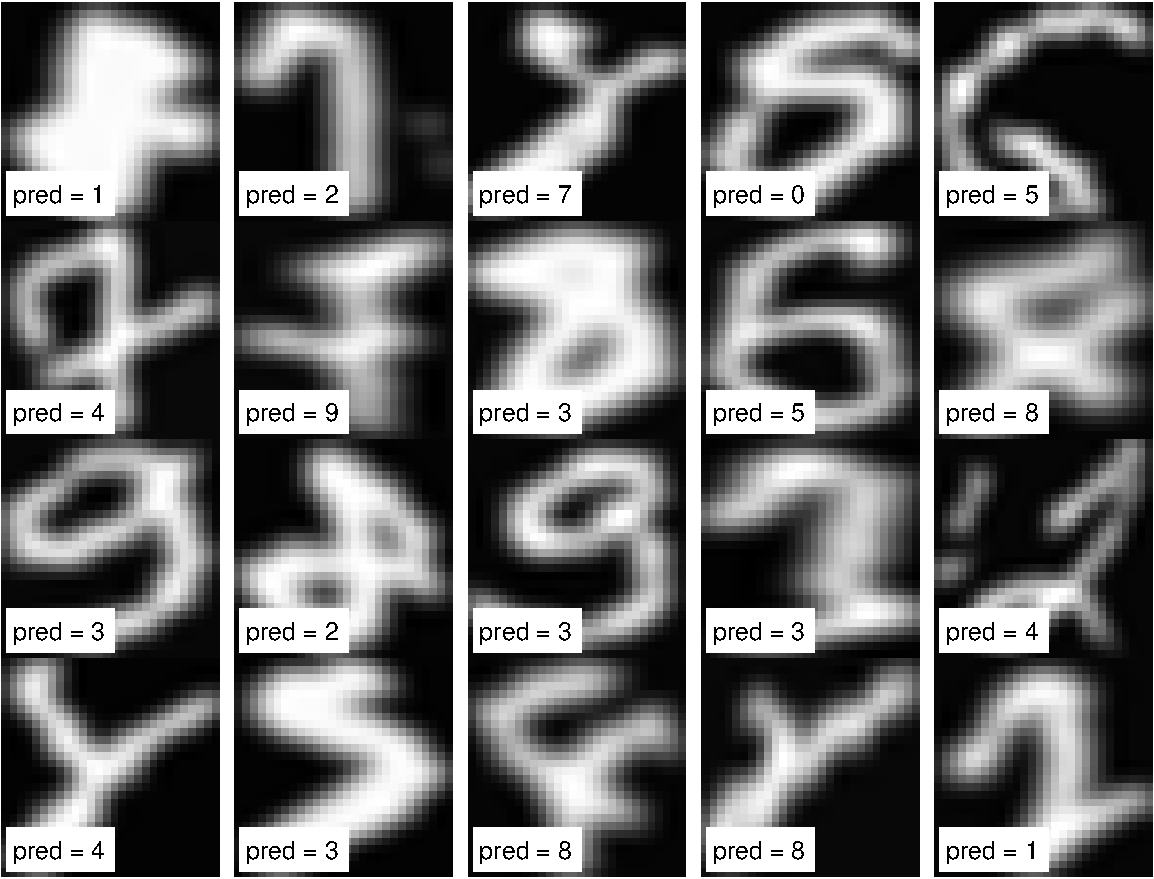
\includegraphics[width=6.7cm]{best_mis}
\caption{Some misclassified samples are unrecognisable even by a human classifier, although the median filter might help us get rid of the outlier elements in the figures like the ! character above but the overall performance drops}
\end{figure}
\section{Conclusion}
On the MNIST problem, some classes are more distinctive than others $\{0,1,3\}$ and although in one vs. one the classes are accurately separated the overall accuracy is generally lower than the one vs rest model with Platt's scaling. As for the chosen kernels the linear, rbf and exponential $\chi_2$ yield better results on the hog space while the rbf is performant on the raw pixels space. Our implementation of the MKL smo is too mush slower than the standard svm smo and generally the elementwise product of kernels represnets the samples similarity better than a linear combination which is the only version we tested with MKL.
\bibliographystyle{acmsiggraph}
\nocite{*}
\bibliography{kernels_refs}

\clearpage
	\begin{algorithm}
	\DontPrintSemicolon
	  \textbf{Inputs:} samples : $(x^{(i)},y^{(i)})_{1\leq i\leq m}$, $tol$ : tolerance, regularization $C\in\mathbb R^m$ \;
	  \textbf{Outputs:} Lagrange multipliers $\alpha$ and the bias $b$\; 
	 \textbf{Initialization:}\;
	 $\alpha = \0$, $b=0$\; 
	 $f = \0$ to store $f(x_i)=\sum_{j=1}^m\alpha_jy^{(j)}K(x^{(j)},x^{(i)})+b$\;
	 $epoch = 0$\;
	 \While{$epoch < 10$}{
	  diff $= 0$ \tcp{number of updated coefficients $\alpha_i$}\;
	  \For{$i=1,...,m$}{
	  compute $E_i = f(i) + b - y^{(i)}$\;
	  \If{$[\:y^{(i)}E_i < -tol\; \wedge \:\alpha_i<C(i)\:] \vee [\:y^{(i)}E_i > tol \:\wedge\: \alpha_i>C(i)\:] $}{
	  select $j\in\{1,...,m\}\backslash\{i\}$\;
	  compute $E_j = f(j) + b - y^{(j)}$\;
	  \tcc{compute bounds of $\alpha_j$ to satisfy the problem's conditions}\;
	  \If{$y^{(i)}=y^{(j)}$}{
	  $L = \max(0,\alpha_i+\alpha_j-C(i))$\;
	  $H = \min(C(j),\alpha_i+\alpha_j)$\;
	  }
	  \Else{
	  $L = \max(0,\alpha_j-\alpha_i)$\;
	  $H = \min(C(j),C(i)+\alpha_j-\alpha_i)$\;
	  }
	  \If{$|L-H|<tol$}{
	   continue to the next $i$\;
	  }
	  $\eta = 2K(i,j)-K(i,i)-K(j,j)$\;
	  \If{$\eta \geq 0$}{
	  continue to the next $i$\; 
	  }
	  \tcc{update $\alpha_i$ and $\alpha_j$}\;
	  }
	  $a_j = \alpha_j-y^{(j)}\frac{E_i-E_j}{\eta}$\; 
	  crop $a_j$ to $[L,H]$\;
	  \If{$|a_j-\alpha_j|< tol$}{
	  continue to the next $i$\;
	  }
	  $a_i = \alpha_i + y^{(i)}y^{(j)}(\alpha_j-a_j)$\;
	  \tcc{choose a suitable bias b}\; 
	  $b_1 = b- E_i - y^{(i)}(a_i-\alpha_i)K(i,i)-y^{(j)}(a_j-\alpha_j)K(i,j)$\;
	  $b_2 = b- E_j - y^{(i)}(a_i-\alpha_i)K(i,j)-y^{(j)}(a_j-\alpha_j)K(j,j)$\;
	  \If{$a_i\in[0,C(i)]$}{$b=b1$\;}
	  \If{$a_j\in[0,C(j)]$}{$b=b2$\;}
	  \If{$a_i\not\in[0,C(i)]\:\wedge\:a_j\not\in[0,C(j)]$}{$b=\frac{b_1+b_2}{2}$\;}
	  update the terms of $f$\;
	  $\alpha_i = a_i$\;
	  $\alpha_j = a_j$\;
	  diff ++\;
	  }
	  \If{ diff = 0}{epoch ++\;}
	  \Else{epoch = 0}
	 }
	\caption{SVM SMO}
	\end{algorithm}


	\begin{algorithm}
	\DontPrintSemicolon
	  \textbf{Inputs:} samples : $(x^{(i)},y^{(i)})_{1\leq i\leq m}$, $tol$ : tolerance, regularization $C\in\mathbb R^m$ \;
	  \textbf{Outputs:} Lagrange multipliers $\alpha$ and the bias $b$\; 
	 \textbf{Initialization:}\;
	 $\alpha = \0$, $b=0$\; 
	 $f = \0$ to store $f(x_i)=\sum_{j=1}^m\alpha_jy^{(j)}K(x^{(j)},x^{(i)})+b$\;
	 $epoch = 0$\;
	 \While{$epoch < 10$}{
	  diff $= 0$ \tcp{number of updated coefficients $\alpha_i$}\;
	  \For{$i=1,...,m$}{
	  compute $E_i = f(i) + b - y^{(i)}$\;
	  \If{$[\:y^{(i)}E_i < -tol\; \wedge \:\alpha_i<C(i)\:] \vee [\:y^{(i)}E_i > tol \:\wedge\: \alpha_i>C(i)\:] $}{
	  select $j\in\{1,...,m\}\backslash\{i\}$\;
	  $s = -y^{(i)}y^{(j)}$\;
	  \tcc{compute bounds of $\alpha_j$ to satisfy the problem's conditions}\;
	  \If{$s=1$}{
	  $L = \max(-\alpha_i,-\alpha_j)$\;
	  $H = \min(C(j)-\alpha_j,C(i)-\alpha_i)$\;
	  }
	  \Else{
	  $L = \max(-\alpha_i,\alpha_j-C(j))$\;
	  $H = \min(C(i)-\alpha_i,\alpha_j)$\;
	  }
	  \If{$|L-H|<tol$}{
	   continue to the next $i$\;
	  }
	  \tcc{compute the optimal step}\;
	  \For{$1\leq l\leq n$}{
	  $A_l=K_l(i,i)+K_l(j,j)-2K_l(i,j)$\;
	  $B_l=y^{(i)}(\alpha\odot Y)^t(K_l(i,:)-K_l(j,:))$\;
	  }
	  \tcc{solve the cubic equation}\;
	  $\Delta^* = \arg\max_{L\leq \Delta \leq U} (1+s)\Delta-...$\;
	  $\phantom{abcdefghijk}\frac{1}{8\lambda}(\sum_{l=1}^n(a_l\Delta^2+2b_l\Delta+c_l)^2)$\;
	  \If{$|\Delta|<tol$}{continue\;}
	  \tcc{update $\alpha_i$ and $\alpha_j$}\;
	  $\alpha_i + = \Delta$\;
	  $\alpha_j + = s\Delta$\;
	  \tcc{update the kernel coefficients $d$}\;
	   $d = d + \frac{1}{2\lambda}\Delta B$\;
	   update the projections $f$\;
	  \tcc{choose a suitable bias b}\; 
	  $b_1 = y^{(i)} - f(i)$\;
	  $b_2 = y^{(j)} - f(j) $\;
	  \If{$a_i\in[0,C(i)]$}{$b=b1$\;}
	  \If{$a_j\in[0,C(j)]$}{$b=b2$\;}
	  \If{$a_i\not\in[0,C(i)]\:\wedge\:a_j\not\in[0,C(j)]$}{$b=\frac{b_1+b_2}{2}$\;}

	  diff ++\;
	 
	  \If{ diff = 0}{epoch ++\;}
	  \Else{epoch = 0}
	 }
	 }
	 }
	\caption{MKL SMO}
	\end{algorithm}


\end{document}